\chapter{WYNIKI TESTÓW}
\label{chapter:wyniki_testow}

\section{Ekran nawigacji} 
Największe trudności pojawiły się podczas implementacji mapy SVG, która miała umożliwiać wygenerowanie sklepu, po który nawigowany będzie użytkownik. Początkowo projekt był realizowany w frameworku NativeScript, który jednak nie oferował wystarczającego wsparcia dla technologii SVG. Brak odpowiednich narzędzi oraz ograniczenia platformy zmusiły nas do przepisania projektu na React Native. Decyzja ta była kluczowa, ponieważ React Native zapewnił znacznie większe możliwości, lepszą elastyczność w zakresie pracy z mapami oraz szersze wsparcie społeczności. Przepisanie projektu przyniosło oczekiwane efekty, a także pozwoliło na bardziej zaawansowaną integrację z zewnętrznymi bibliotekami.

\section{Interfejs mapy sklepów} 
Jednym z najbardziej satysfakcjonujących rezultatów testów był interfejs mapy sklepów. Po wdrożeniu i testach w środowisku produkcyjnym mapa okazała się niezwykle wygodna i intuicyjna dla użytkowników. Funkcjonalności, takie jak automatyczne centrowanie na najbliższym sklepie czy możliwość łatwego nawigowania między różnymi lokalizacjami, zostały bardzo dobrze ocenione. Testy z udziałem rzeczywistych użytkowników potwierdziły, że interfejs jest nie tylko estetyczny, ale także funkcjonalny.

\section{Obsługa niewidomych} 
Równie istotnym elementem były testy komend głosowych, które przeprowadzaliśmy w warunkach symulujących rzeczywiste użycie aplikacji przez osoby niedowidzące. W trakcie testów celowo zamykaliśmy oczy, aby sprawdzić, czy dzięki komendom głosowym możliwe jest osiągnięcie zamierzonych celów, takich jak przejście na odpowiedni widok czy dodanie produktu do koszyka. Efekty końcowe przeszły nasze oczekiwania – system rozpoznawania mowy zareagował poprawnie na większość poleceń, a intuicyjne komunikaty głosowe pozwalały na sprawne wykonywanie działań w aplikacji. Tego rodzaju testy pozwoliły na optymalizację obsługi głosowej, zwiększając jej precyzję oraz dostępność dla użytkowników.

\section{API Wit.ai}
\label{section:witai}
W celu przetestowania działania modelu językowego opracowanego na platformie Wit.ai przeprowadzono testy na przykładowych zdaniach. Do testów przygotowano zdania, które użytkownik aplikacji mógłby zadać. Poniżej przedstawiono pytania wykorzystane pdczas testów:

\begin{itemize}
    \item Add bread from biedronka to cart
    \item Add bread to cart
    \item Go to cart
    \item What is this?
\end{itemize}


W celu przetestowania przepływu interaktywnego, w którym system oczekuje od użytkownika odpowiedzi, w celu zrealizowania akcji, wykorzystano zapytanie \textit{Add bread from biedronka to cart}. System prawidłowo rozpoznał encję \textit{product} oraz \textit{store}. System pyta użytkownika, czy dodany ma zostać tylko jeden bochenek chleba. Po otrzymaniu pozytywnej odpowiedzi, system zwraca do aplikacji informację, że należy dodać dany produkt do koszyka. W przypadku gdyby któraś z encji nie zostałą rozpoznana, system zadałby pytanie z prośbą o uzupełnienie kontekstu. Przykład takiego zachowania przedstawiono na rysunku \ref{fig:witai_context_example}.
\begin{figure}[H]
    \centering
    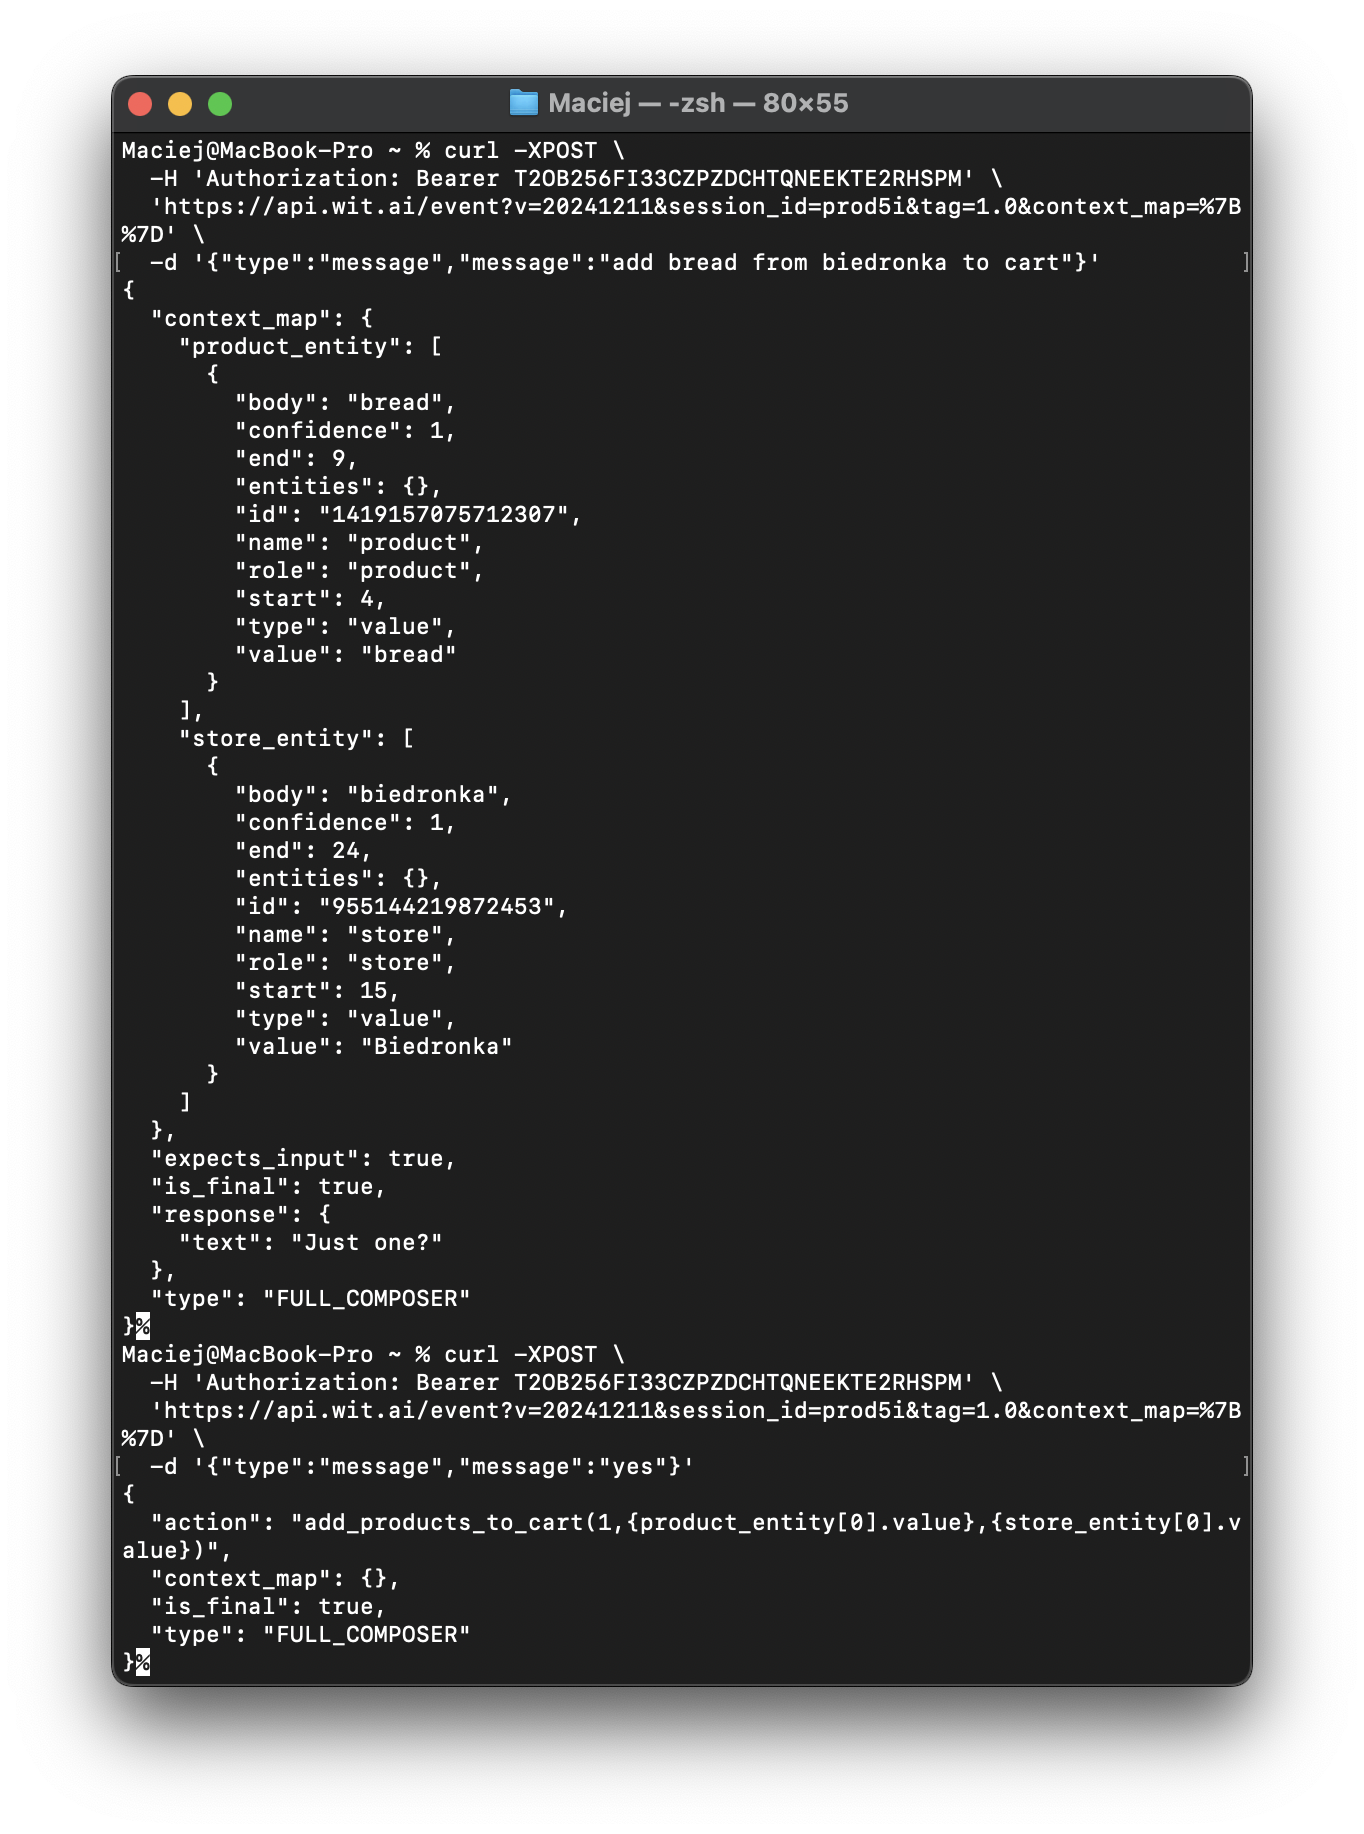
\includegraphics[width=0.8\textwidth]{images/witai_complex_convo.png}
    \caption{Przykład kompleksowej konwersacji z systemem Wit.ai}
    \label{fig:witai_complex_convo}
\end{figure}

\begin{figure}[H]
    \centering
    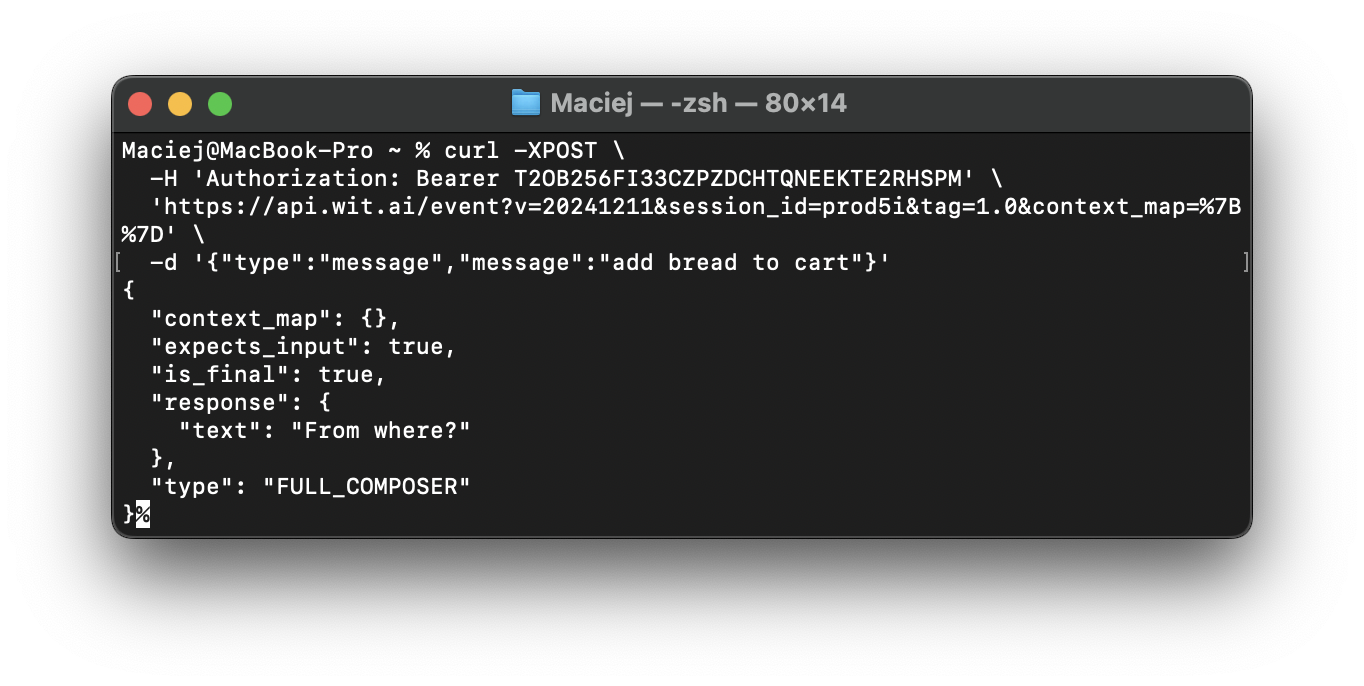
\includegraphics[width=0.8\textwidth]{images/witai_context_example.png}
    \caption{Przykład pytania systemu Wit.ai o uzupełnienie kontekstu}
    \label{fig:witai_context_example}
\end{figure}

Jak widać na rysunku \ref{fig:witai_context_example}, system zapytał użytkownika o uzupełnienie kontekstu, gdyż nie otrzymał informacji na temat sklepu.

\begin{figure}[H]
    \centering
    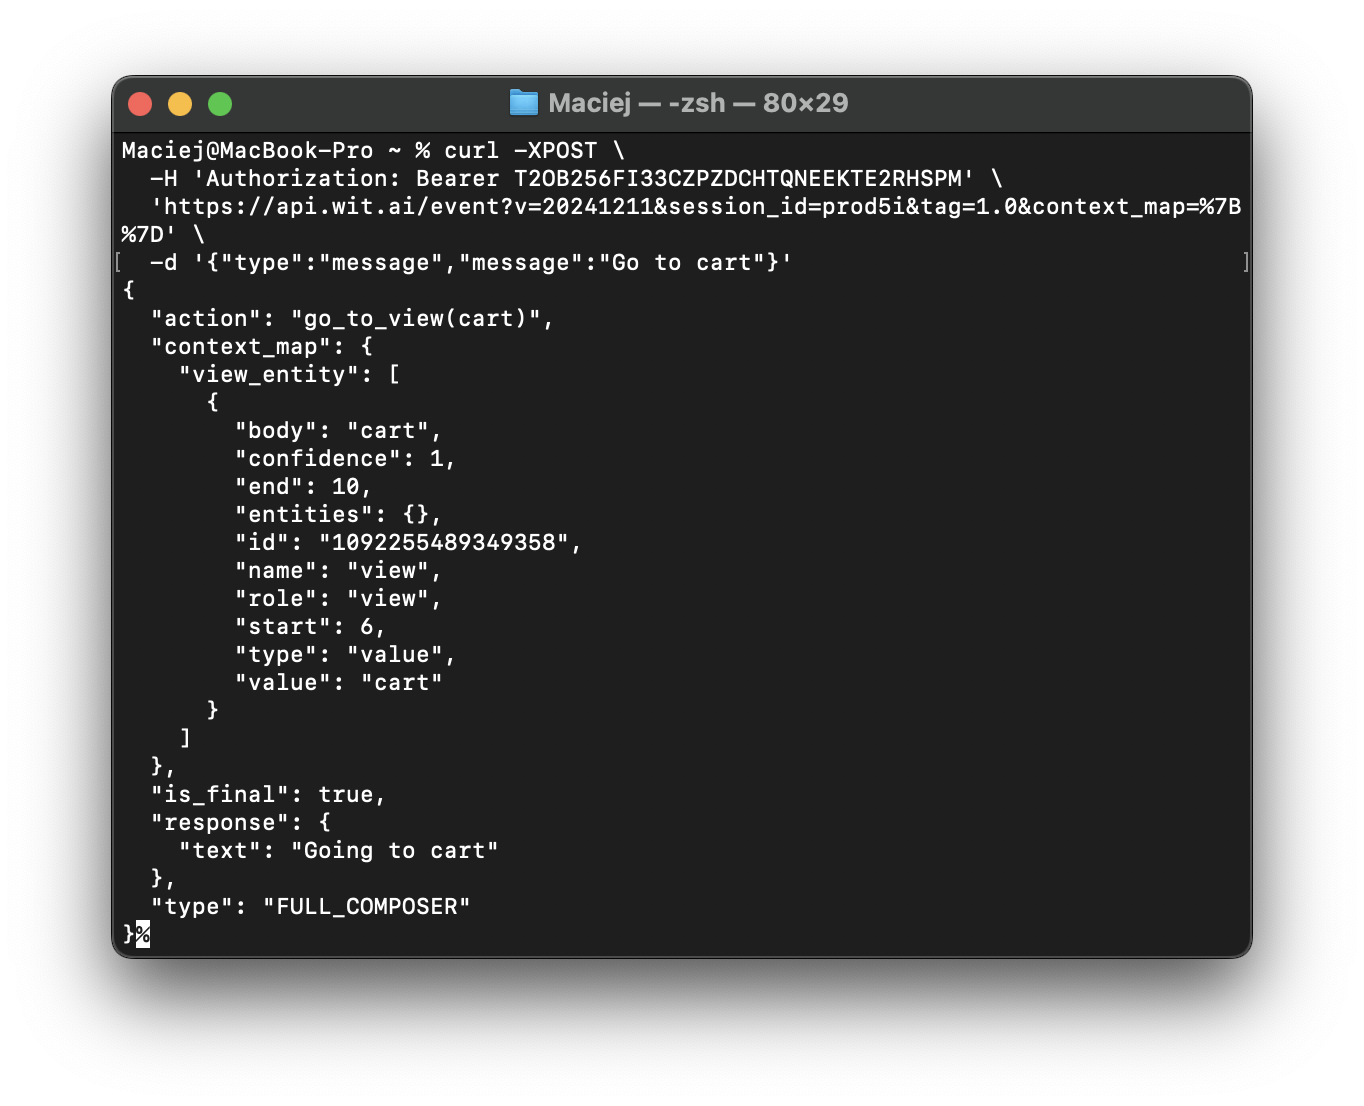
\includegraphics[width=0.8\textwidth]{images/witai_go_to_cart.png}
    \caption{Przykład przejścia do widoku koszyka}
    \label{fig:witai_cart_example}
\end{figure}

Na rysunku \ref{fig:witai_cart_example} przedstawiono przykład przejścia do widoku koszyka. System poprawnie zrozumiał zapytanie i zwrócił odpowiedź, że użytkownik chce przejść do koszyka.

\begin{figure}
    \centering
    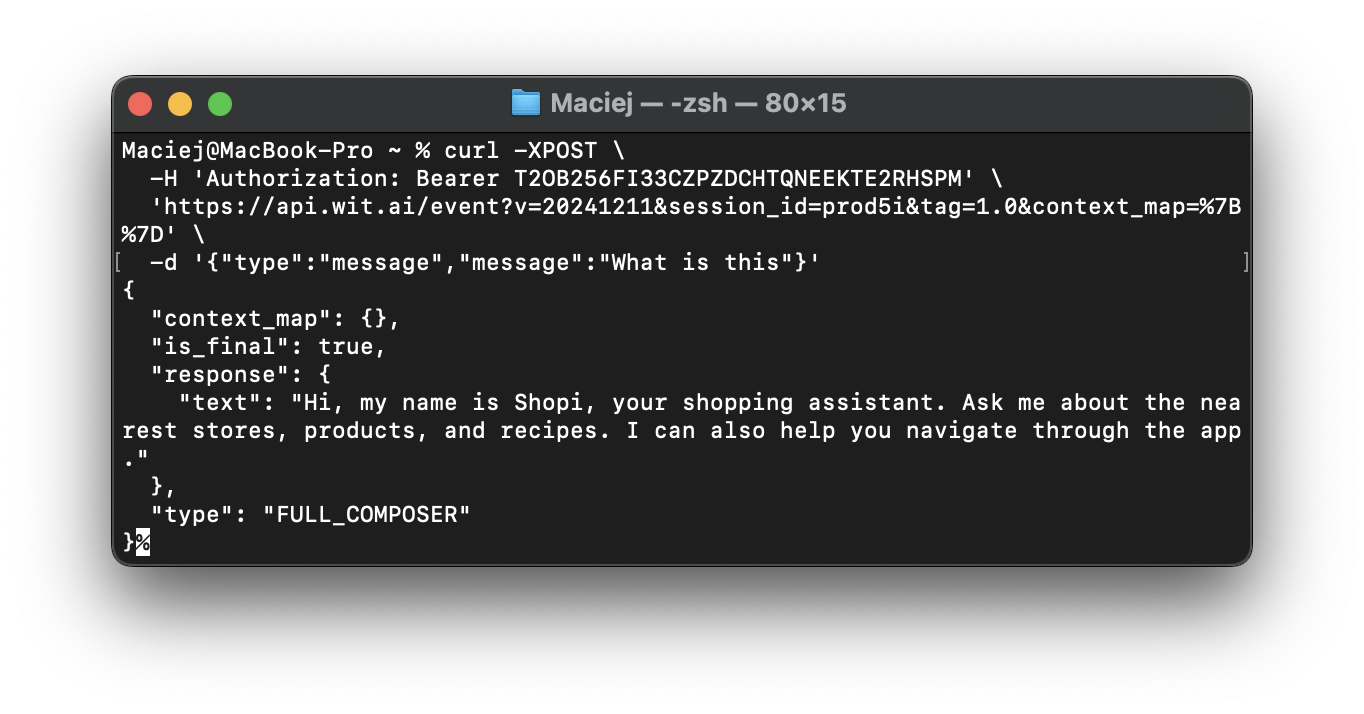
\includegraphics[width=0.8\textwidth]{images/witai_what_is_this.png}
    \caption{Przykład zapytania o nazwę produktu}
    \label{fig:witai_what_is_this}
\end{figure}

Na rysunku \ref{fig:witai_what_is_this} przedstawiono przykład zapytania zakłopotanego użytkownika, który nie wie, co to jest. System w odpowiedzi na takie pytanie, przedstawił się, co jest oczekiwanym zachowaniem.


\section{Testy pozycjonowania w korytarzu (symulacja warunków sklepowych)}
\label{subsec:testy_pozycjonowania_korytarz}

W celu oceny dokładności i stabilności systemu pozycjonowania przeprowadzono testy w warunkach domowych, korzystając z korytarza o długości około 15 m, co miało symulować jednoliniową strukturę alejki sklepowej. Wzdłuż korytarza umieszczono nadajniki BLE w regularnych odstępach (co 2--3 m), a pomiary wartości RSSI uśredniano i wygładzano filtrem Kalmana.

\paragraph{Scenariusz testów:} 
\begin{itemize}
    \item \textbf{Pozycjonowanie statyczne:} Tester pozostawał w jednym miejscu (np. w połowie korytarza), a system na bieżąco aktualizował pozycję. Uzyskano stabilność pozycji z błędem rzędu 5-15 cm.
    \item \textbf{Pozycjonowanie w ruchu:} Tester poruszał się z prędkością około 1 m/s na całej długości korytarza. Średni błąd wynosił 15--30 cm. Filtr Kalmana skutecznie niwelował drobne fluktuacje RSSI.
    \item \textbf{Wpływ drobnych zakłóceń:} Nawet obecność niewielkich przeszkód (metalowe przedmioty, meble) rzadko pogarszała dokładność powyżej 30 cm.
\end{itemize}

Uzyskane wyniki wskazują, że w kontrolowanych warunkach możliwe jest osiągnięcie bardzo dobrej dokładności pozycjonowania, co stanowi solidną podstawę przed wdrożeniem systemu w bardziej złożonym środowisku, takim jak sklep.


\section{Testy wyznaczania trasy na wygenerowanych grafach}
\label{subsec:testy_trasowania_grafy}

W celu oceny efektywności i skalowalności algorytmów trasowania (algorytm Dijkstry, heurystyka 2-opt) przeprowadzono testy w środowisku symulacyjnym. Wygenerowano różne grafy, odwzorowujące układy alejek sklepowych o zróżnicowanej liczbie wierzchołków (od kilkunastu do kilkuset) i połączeń.

\paragraph{Scenariusz testów:} 
\begin{itemize}
    \item \textbf{Małe grafy (20--30 wierzchołków):} Czas wyznaczenia najkrótszych ścieżek i optymalizacji 2-opt był pomijalnie mały (ułamki milisekund).
    \item \textbf{Średnie grafy (50--100 wierzchołków):} Obliczenia trwały kilka milisekund. Aktualizacja trasy w reakcji na zmiany celu lub pozycji użytkownika zachodziła niemal natychmiast.
    \item \textbf{Duże grafy (kilkaset wierzchołków):} Czas obliczeń rzadko przekraczał 100--200 ms, co nadal jest akceptowalne w kontekście systemu nawigacji sklepowej.
\end{itemize}

Testy symulacyjne potwierdziły wysoką wydajność i elastyczność przyjętych algorytmów trasowania. Nawet dla bardziej złożonych układów, typowych dla dużych sklepów, system jest w stanie szybko obliczyć i zoptymalizować trasę, zapewniając responsywną i interaktywną nawigację w czasie rzeczywistym.
